\section{\bench}

\begin{figure}[t]
  \centering
  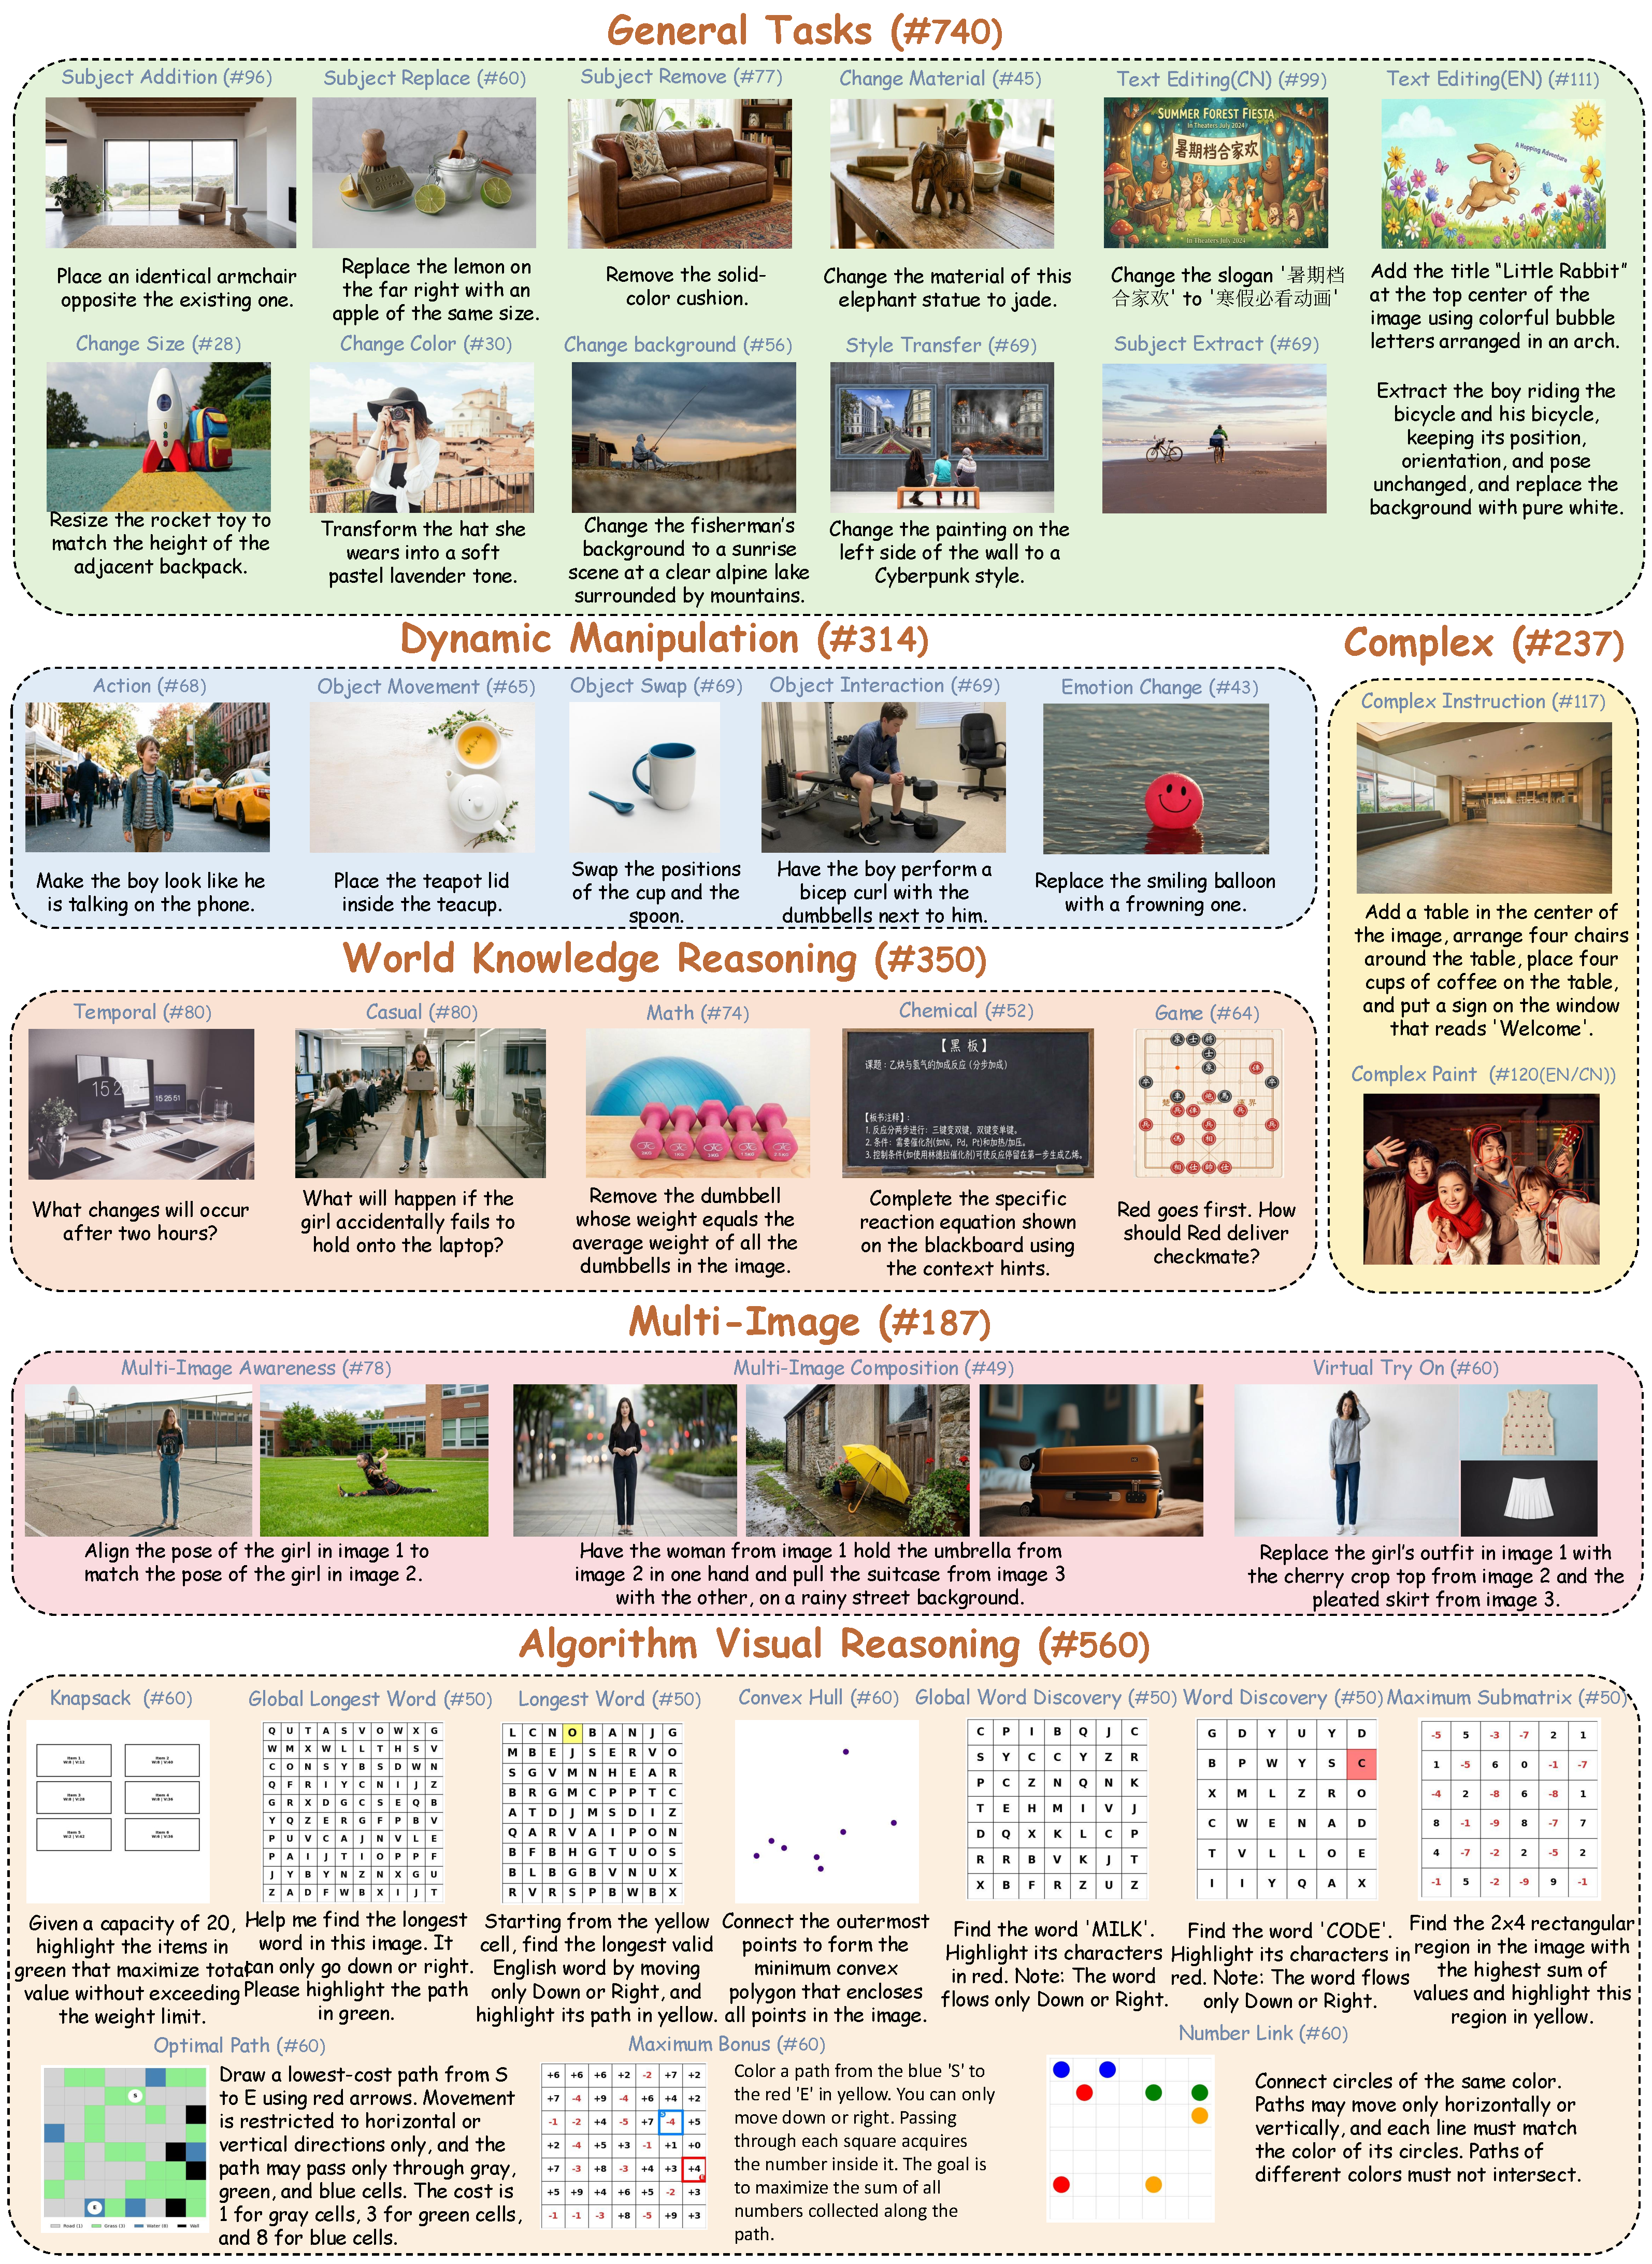
\includegraphics[width=0.8\linewidth]{image/NIPS_Gallery_num3.pdf}
   
  \caption{\textbf{{\bench}} covers 36 diverse image editing tasks, spanning single-image and multi-image settings as well as general editing and algorithmic visual reasoning. Each panel shows a representative example for a task type, with the number of examples (\#) indicated.}
  \label{fig:gallery}
  \vspace{-1.0em}
\end{figure}

\subsection{Task Taxonomy}

\textbf{General Tasks.} 
General tasks evaluate the fundamental image editing capabilities of models, focusing on instruction understanding and accurate execution across both global and local editing scenarios. Global editing includes tasks such as \textit{style transfer} and \textit{background transformation}, while local editing extends beyond conventional operations like addition, removal, and replacement to more fine-grained edits.
As illustrated in Figure~\ref{fig:gallery}, we introduce a novel \textit{Copy} task, which requires models to duplicate an existing object within the input image while preserving its visual attributes and maintaining spatial coherence. We further include challenging tasks such as \textit{change size}, which evaluate the ability to manipulate object scale and spatial relationships. Together, these tasks provide a comprehensive evaluation of general image editing capabilities at both global and object levels.

\textbf{Dynamic Manipulation Tasks.}
Dynamic Manipulation tasks evaluate a model's ability to perform object-level dynamic edits in real-world scenes, focusing on actions, movements, emotional changes, and inter-object interactions. Unlike general editing tasks, this category emphasizes dynamic scene understanding and interaction modeling.
Specifically, this category includes five subtasks: (1) \textit{Action}, which modifies object motion; (2) \textit{Emotion Change}, which alters object expressions or affective states; (3) \textit{Object Movement}, which repositions objects within the scene; (4) \textit{Object Swap}, which exchanges attributes such as appearance, color, or state between objects; and (5) \textit{Object Interaction}, which evaluates the modeling of interactions among multiple objects.


\textbf{World Knowledge Reasoning Tasks.}
These tasks evaluate a model's ability to leverage real-world knowledge to infer and execute intended edits. We define five representative subtasks: (1) \textit{Temporal Reasoning}, which involves reasoning about past and future changes over time; (2) \textit{Causal Reasoning}, which evaluates understanding of object changes under external conditions; (3) \textit{Game Reasoning}, which requires reasoning about game rules and states; (4) \textit{Math Reasoning}, which tests mathematical reasoning ability; and (5) \textit{Chemical Reasoning}, which involves understanding chemical phenomena and reactions.
These tasks evaluate models' abilities in temporal, causal, and domain-specific reasoning for complex image editing scenarios.

\textbf{Algorithmic Visual Reasoning Tasks.}  
Algorithmic visual reasoning tasks evaluate whether models can interpret visual inputs and perform multi-step reasoning to execute corresponding edits. This category includes ten task types, such as \textit{Optimal Path Identification}, \textit{Convex Hull Identification}, \textit{Maximum Submatrix Sum Identification}, and \textit{Knapsack Selection}. These tasks require models to understand visual structures, reason over them, and faithfully render the results through image editing, providing a challenging benchmark for deep visual reasoning in image editing.

\textbf{Multi-Image Tasks.} 
Multi-image tasks evaluate a model's ability to understand and integrate multiple input images for image editing. Beyond \textit{Multi-Image Composition} and \textit{Virtual Try-On}, we introduce a novel task termed \textit{Multi-Image-Aware Editing}, where models edit a target image based on fine-grained attributes extracted from reference images, such as object properties, actions, orientations, and colors. These tasks comprehensively evaluate models' abilities to understand, transfer, and manipulate visual information across multiple images.

\textbf{Complex Tasks.} 
Complex tasks evaluate a model's ability to handle compound instructions involving multiple editing intents. Unlike single-step editing tasks, these tasks require coherent execution of multiple edits within the source image.
We further introduce \textit{Complex Paint}, a multimodal editing task that incorporates visual guidance directly into the source image through cues such as arrows, circles, and cross marks. This setting better reflects real-world interactive editing scenarios, where users combine textual instructions with visual indications to specify complex edits.
These tasks provide a more rigorous evaluation of compositional and multimodal image editing capabilities.

\begin{figure}[t]
  \centering
  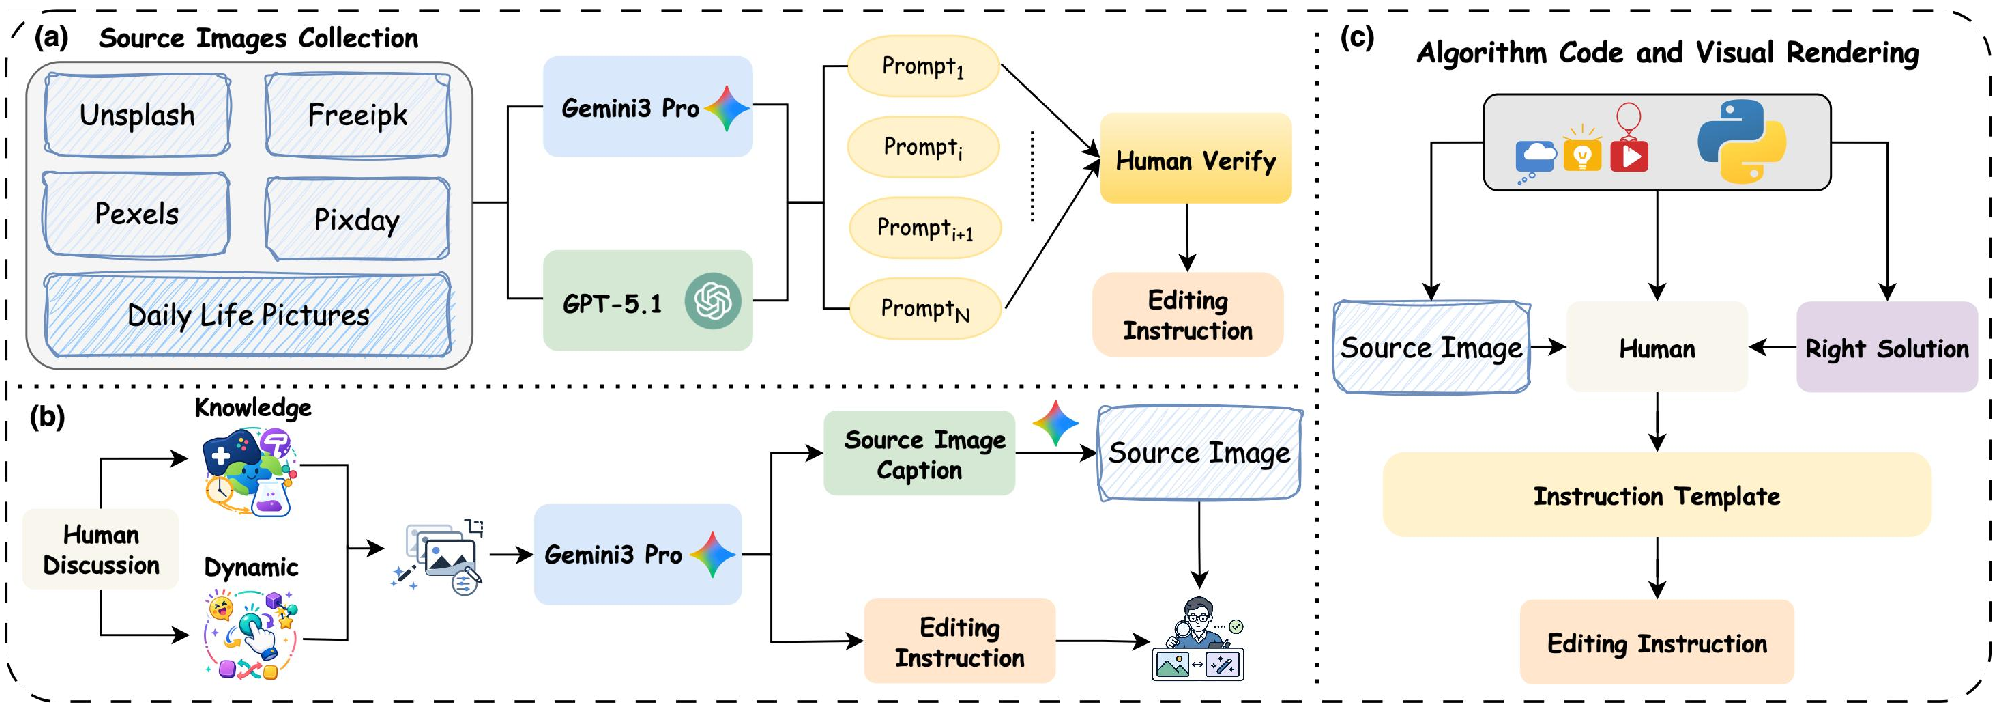
\includegraphics[width=0.95\textwidth]{image/data_construction22.pdf}
   
  \caption{\textbf{Overview of the source data construction pipelines in \bench.}
(a) General and Complex tasks.
(b) Dynamic Manipulation, World Knowledge Reasoning, and Multi-Image tasks.
(c) Algorithmic Visual Reasoning tasks.}
  \label{Fig: Data Construction}
  \vspace{-1em}
\end{figure}


% Summary
\subsection{Benchmark Construction}
The source data in {\bench} consists of original images and executable editing instructions. As illustrated in Figure~\ref{Fig: Data Construction}, we adopt three data construction strategies tailored to different task categories.
For General and Complex tasks, original images are collected from online resources and real-world photographs, while editing instructions are generated with Gemini 3 Pro~\cite{gemini3pro} and GPT-5.1~\cite{gpt4o20250325}, followed by human verification. For Dynamic Manipulation, World Knowledge Reasoning, and Multi-Image tasks, image-editing experts design challenging yet realistic scenarios, describe the desired source images, and construct bilingual editing instructions in Chinese and English. The source images are then generated from enhanced prompts refined by Gemini 3 Pro~\cite{gemini3pro}. For Algorithmic Visual Reasoning tasks, we programmatically generate source images using Python and derive ground-truth annotations from algorithmic solutions.
To ensure consistency and clarity, we design unified instruction templates for each task category that specify task requirements and intended outcomes. All samples are further reviewed by multiple human experts to ensure data quality. More details are provided in Appendix~\ref{supp: Edit-Compass Data Construction}.

\subsection{Evaluation Pipeline}
Accurately evaluating diverse image editing tasks in a human-aligned manner remains challenging, especially for instruction adherence and visual consistency. To address this, we structure the evaluation around three core dimensions: \textbf{Instruction Awareness}, \textbf{Visual Consistency}, and \textbf{Visual Quality}. Based on these dimensions, we design an MLLM-as-judge evaluation pipeline that produces both scalar scores and fine-grained rationales. For reasoning-intensive tasks, the rationale further includes the expected ground-truth outcome, improving evaluation accuracy and interpretability. More details are provided in Appendix~\ref{supp: Evaluation pipeline}.

\textbf{Dimension 1: Instruction Awareness.}
This dimension evaluates whether the edited image correctly follows the instruction and reflects the intended change. It consists of two dynamic subcomponents: \textit{Instruction Following} and \textit{World Knowledge Awareness}. Instruction following assesses whether the model correctly identifies the target object, applies the required attribute or spatial modification, and satisfies explicit constraints. World knowledge awareness evaluates whether the model incorporates relevant real-world knowledge and visual cues to infer implicit editing intent.

\textbf{Dimension 2: Visual Consistency.}
This dimension measures whether visual content unrelated to the requested edit is preserved. It includes \textit{Unedited Region Consistency (URC)} and \textit{Identity Consistency}. URC evaluates whether non-edited regions remain unchanged at both local and global levels. Identity consistency assesses whether the edited object preserves attributes irrelevant to the requested modification, avoiding unintended changes in appearance, structure, or identity.

\textbf{Dimension 3: Visual Quality.}
This dimension evaluates whether the edited image is visually plausible, coherent, and artifact-free. It considers naturalness, structural fidelity, artifact severity, distortion, and text legibility when applicable.




\section{\rmbench}
{\rmbench} is designed to systematically evaluate reward models for image editing. It contains $2,251$ preference pairs, each consisting of an editing instruction and two candidate edited images. We evaluate reward models using the same rubric-based judging framework as {\bench}, enabling consistent assessment across image editing models and reward models. This also allows us to examine the robustness and generality of our evaluation prompts. The construction of {\rmbench} follows two stages: sampling (Section~\ref{Sampling Stage}) and human annotation (Section~\ref{Reward Model Benchmark Human Annotation}).



\subsection{Sampling Stage}
\label{Sampling Stage}
We use {\bench} as the source data for constructing {\rmbench}, as its diverse and executable editing instructions provide broad coverage of realistic editing scenarios. To better reflect reward modeling during RL optimization, we simulate the sampling process with a FlowGRPO-inspired strategy~\cite{liu2025flow} and introduce stochasticity through stochastic differential equations~\cite{song2020score}.
Specifically, we sample candidate outputs from six image editing models and control the denoising steps to ensure visually clear and valid results. For tasks involving world knowledge or complex reasoning, where open-source models often show limited capability, we further expand the sampling pool to ten diverse open-source and proprietary models to improve task diversity and coverage. Additional implementation details are provided in Appendix~\ref{supp: EditReward-Compass Data Construction}.

\subsection{Human Annotation Stage}
\label{Reward Model Benchmark Human Annotation}
To ensure the quality of {\rmbench}, we employ a two-stage human annotation pipeline to select preference pairs along multiple dimensions, including instruction adherence, visual consistency, and visual quality. Given the complexity of image editing evaluation, {\rmbench} places particular emphasis on instruction adherence and visual consistency. The annotation process involves eight human experts in image editing.
In the first stage, three annotators independently review sampled outputs to construct candidate preference pairs. Ambiguous cases are flagged and resolved through discussion, leading to either consensus decisions or sample removal. In the second stage, five annotators conduct fine-grained verification of the selected pairs, checking both task validity and preference correctness. A pair is retained only when all five annotators reach unanimous agreement, ensuring high annotation consistency.

\begin{table*}[t]
    \centering
    
    \caption{
    \textbf{Main results on {\bench} under English instructions.} The best results are marked in \textbf{bold} for
    {\color[HTML]{F88825} open-} and {\color[HTML]{319B62} closed-} models, respectively.}
    \label{tab:Image Editing Bench Main Results_EN}
    \resizebox{\linewidth}{!}{
        \begin{tabular}{lc|ccc|ccc|ccc|ccc|ccc|ccc|c}
            \toprule
            \multirow{2}{*}{Model} & \multirow{2}{*}{Multi-Img}
            & \multicolumn{3}{c}{\textbf{General}}
            & \multicolumn{3}{c}{\textbf{Dynamic Manipulation}}
            & \multicolumn{3}{c}{\textbf{World Knowledge}}
            & \multicolumn{3}{c}{\textbf{Visual Reasoning}}
            & \multicolumn{3}{c}{\textbf{Multi Image }}
            & \multicolumn{3}{c}{\textbf{Complex}}
            & \textbf{Overall} \\
            &
            & $\mathcal{IA}\uparrow$ & $\mathcal{VC}\uparrow$ & $\mathcal{VQ}\uparrow$
            & $\mathcal{IA}\uparrow$ & $\mathcal{VC}\uparrow$ & $\mathcal{VQ}\uparrow$
            & $\mathcal{IA}\uparrow$ & $\mathcal{VC}\uparrow$ & $\mathcal{VQ}\uparrow$
            & $\mathcal{IA}\uparrow$ & $\mathcal{VC}\uparrow$ & $\mathcal{VQ}\uparrow$
            & $\mathcal{IA}\uparrow$ & $\mathcal{VC}\uparrow$ & $\mathcal{VQ}\uparrow$
            & $\mathcal{IA}\uparrow$ & $\mathcal{VC}\uparrow$ & $\mathcal{VQ}\uparrow$
            & \cellcolor[HTML]{C8C8C8}\textbf{AVG} \\ \hline

InstructPix2Pix~\cite{brooks2023instructpix2pix} & \ding{55}
& 1.98 & 1.34 & 2.33 & 1.72 & 1.61 & 2.23 & 1.51 & 1.56
& 2.57 & 1.09 & 1.66 & 3.26 & - & - & - & 1.91 & 1.15 &  2.07
& \cellcolor[HTML]{C8C8C8}1.19 \\

UltraEdit~\cite{zhao2024ultraedit} & \ding{55}
& 2.23 & 1.80 & 2.44 & 1.82 & 2.37 & 2.44 & 1.56 & 2.32 & 2.89
& 1.04 & 3.34 & 3.71 & - & - & - & 1.82  & 1.31 & 2.11
& \cellcolor[HTML]{C8C8C8}1.28 \\

AnyEdit~\cite{yu2025anyedit} & \icohalfno 
& 2.05 & 2.36 & 2.47  & 1.61 & 2.73 & 2.48 & 1.45 & 2.81
& 2.95 & 1.03 & 3.21 & 3.44 & - & - & - & 1.34 & 1.78 & 2.07
& \cellcolor[HTML]{C8C8C8}1.31 \\

MagicBrush~\cite{zhang2023magicbrush} & \ding{55}
& 2.21  & 2.11 & 2.28 & 1.75 & 2.42 & 2.29 & 1.51 & 2.58 & 2.49  & 1.05
& 1.69 & 2.37 & - & - & - & 1.53 & 1.66 & 2.10
& \cellcolor[HTML]{C8C8C8}1.33 \\


FLUX.1 Kontext Dev~\cite{labs2025flux} & \ding{55}
& 3.53 & 2.98 & 3.09 & 2.41 & 2.93 & 2.81 & 1.65 & 3.22 & 3.32 & 1.27
& 3.98 & \color[HTML]{F88825}\textbf{4.78} & - & - & - & 2.41 & 2.32 & 2.63
& \cellcolor[HTML]{C8C8C8}1.93 \\

FLUX.2 Dev~\cite{flux-2-2025} & $\checkmark$
& 4.24 & 4.16 & \color[HTML]{F88825}\textbf{3.96} & 3.23 & \color[HTML]{F88825}\textbf{4.36} & \color[HTML]{F88825}\textbf{3.36} &  2.05 & 3.85 & \color[HTML]{F88825}\textbf{3.71}
& 1.42 & 2.85 & 4.56 & 3.16 & 4.13 & \color[HTML]{F88825}\textbf{3.14} & 2.62 & \color[HTML]{F88825}\textbf{4.32} & \color[HTML]{F88825}\textbf{3.54}
& \cellcolor[HTML]{C8C8C8} 2.61 \\
\hline

OneCAT~\cite{li2025onecat} & \ding{55}
& 2.23 & 1.12 & 2.12
& 1.67 & 1.26 & 2.15
& 1.41 & 1.29 & 2.09
& 1.02 & 1.05 & 2.06
& - & - & -
& 1.79 & 1.03 & 1.99
& \cellcolor[HTML]{C8C8C8}1.21 \\

Lumina-DiMOO~\cite{xin2025lumina} & \ding{55}
& 2.37 & 2.00 & 2.33
& 1.73 & 2.31 & 2.40
& 1.50 & 2.89 & 2.93
& 1.09 & 2.08 & 2.83
& - & - & -
& 1.70 & 1.54 & 2.08
& \cellcolor[HTML]{C8C8C8}1.33 \\

Nextstep-V1~\cite{han2025nextstep} & \ding{55}
& 3.31 & 1.73 & 2.29
& 2.35 & 1.81 & 2.23
& 1.74 & 1.81 & 2.28
& 1.11 & 1.02 & 2.08
& - & - & -
& 2.14 & 1.22 & 2.09
& \cellcolor[HTML]{C8C8C8}1.45 \\

InternVL-U~\cite{tian2026internvl} & \ding{55}
& 3.84 & 2.13 & 2.69
& 2.54 & 1.91 & 2.40
& 1.82 & 2.35 & 2.69
& 1.18 & 1.91 & 2.66
& - & - & -
& 2.42 & 1.38 & 2.22
& \cellcolor[HTML]{C8C8C8}1.59 \\

UniWorld-V1~\cite{lin2025uniworld} & $\checkmark$
& 2.94 & 3.19 & 3.09 & 1.85 & 3.34 & 2.93 & 1.47 & 3.17 & 3.27
& 1.06 & 1.59 & 3.59 & 1.74 & 2.02 & 2.81 & 1.74 & 2.65 & 2.41
& \cellcolor[HTML]{C8C8C8}1.71 \\

HiDream-E1~\cite{cai2025hidream} & \ding{55}
& 3.29 & 2.42 & 2.75
& 2.66 & 2.65 & 2.68
& 1.77 & 2.54 & 2.80
& 1.22 & 2.55 & 3.75
& - & - & -
& 2.26 & 1.59 & 2.14
& \cellcolor[HTML]{C8C8C8}1.76 \\


ChronoEdit~\cite{wu2025chronoedit} & \ding{55}
& 2.63 & 3.63 & 3.49
& 2.85 & 3.84 & 3.22
& 1.61 & 3.26 & 3.35
& 1.15 & 1.87 & 3.45
& - & - & -
& 1.97 & 3.00 & 2.83
& \cellcolor[HTML]{C8C8C8}1.85 \\


OmniGen2~\cite{wu2025omnigen2} & $\checkmark$
& 3.33 & 3.34 & 3.12
& 2.47 & 3.70 & 3.19
& 1.53 & 3.33 & 3.55
& 1.11 & 2.51 & 3.69
& 2.55 & 1.77 & 2.65
& 2.27 & 2.73 & 2.73
& \cellcolor[HTML]{C8C8C8}1.88 \\

DeepGen 1.0~\cite{wang2026deepgen} & \ding{55}
& 3.85 & 2.45 & 2.94
& 2.88 & 2.50 & 2.62
& 2.30 & 2.68 & 3.13
& \color[HTML]{F88825}\textbf{1.57} & \color[HTML]{F88825}\textbf{4.33} & 4.44
& - & - & -
& 2.66 & 1.68 & 2.28
& \cellcolor[HTML]{C8C8C8}1.91 \\

UniReason1.0~\cite{wang2026unireason} & $\checkmark$
& 3.58 & 2.82 & 2.81
& 3.31 & 3.09 & 2.71
& 2.32 & 3.05 & 2.90
& 1.42 & 4.08 & 3.20
& 1.90 & 1.59 & 2.77
& 2.55 & 1.52 & 2.30
& \cellcolor[HTML]{C8C8C8}1.92 \\


Bagel-Think~\cite{deng2025emerging} & $\checkmark$
& 3.52 & 3.92 & 3.14
& 2.55 & 4.04 & 3.15
& 2.22 & 3.09 & 3.27
& 1.21 & 3.25 & 3.48
& 1.85 & 2.01 & 3.03
& 2.19 & 3.35 & 2.89
& \cellcolor[HTML]{C8C8C8}2.08 \\



Bagel~\cite{deng2025emerging} & $\checkmark$
& 3.80 & 4.00 & 3.16
& 2.49 & 3.84 & 2.99
& 1.78 & 3.59 & 3.38
& 1.21 & 3.28 & 3.83
& 1.86 & 2.03 & 3.06
& 2.30 & 2.99 & 2.65
& \cellcolor[HTML]{C8C8C8}2.10 \\

Unipic3~\cite{wei2026skywork} & $\checkmark$
& 4.22 & 3.85 & 3.52
& 3.25 & 3.58 & 3.03
& 2.02 & 3.37 & 3.07
& 1.20 & 2.47 & 3.73
& 3.00 & 3.04 & 2.72
& 2.76 & 2.63 & 2.74
& \cellcolor[HTML]{C8C8C8}2.35 \\

UniWorld-V2~\cite{li2025uniworld} & $\checkmark$
& 4.39 & 4.04 & 3.74
& 3.64 & 3.64 & 3.03
& 2.22 & 3.27 & 3.25
& 1.21 & 2.27 & 3.64
& 3.05 & 3.13 & 2.82
& 2.91 & 2.73 & 2.82
& \cellcolor[HTML]{C8C8C8}2.53 \\

Step1X-Edit-v1p2~\cite{liu2025step1x} & \ding{55}
& 4.26 & 4.31 & 3.64
& 3.16 & 4.15 & 3.12
& 2.30 & \color[HTML]{F88825}\textbf{4.09} & 3.49
& 1.26 & 2.72 & 4.41
& - & - & -
& 2.94 & 3.33 & 2.81
& \cellcolor[HTML]{C8C8C8}2.58 \\


Longcat-Image-Edit~\cite{team2025longcat} & \ding{55}
& 4.51 & \color[HTML]{F88825}\textbf{4.48} & 3.90
& 3.54 & 4.14 & 3.38
& 1.98 & 3.94 & 3.49
& 1.31 & 3.26 & 4.21
& - & - & -
& 2.72 & 3.31 & 3.19
& \cellcolor[HTML]{C8C8C8}2.65 \\

EMU3.5~\cite{cui2025emu3} & $\checkmark$
& 4.45 & 4.00 & 3.68 & 3.78 & 3.79 & 3.23 & \color[HTML]{F88825}\textbf{2.60} & 3.55 & 3.33
& 1.43 & 3.54 & 3.83 & \color[HTML]{F88825}\textbf{3.46} & 3.43 & 2.89 & 2.71 & 3.28 & 2.93
& \cellcolor[HTML]{C8C8C8}2.66 \\


JoyAI-Image-Edit~\cite{joyaiimage2026} & \ding{55}
& 4.56 & 4.35 & 3.61
& 3.65 & 4.14 & 3.17
& 2.35 & 3.87 & 3.46
& 1.41 & 2.56 & 4.38
& - & - & -
& \color[HTML]{F88825}\textbf{3.00} & 3.41 & 2.87
& \cellcolor[HTML]{C8C8C8}2.68 \\

Qwen-Image-Edit-2511~\cite{wu2025qwen} & $\checkmark$
& \color[HTML]{F88825}\textbf{4.61} & 4.39 & 3.75
& \color[HTML]{F88825}\textbf{3.81} & 3.93 & 3.16
& 2.33 & 3.56 & 3.25
& 1.26 & 2.53 & 4.09
& 3.27 & \color[HTML]{F88825}\textbf{3.55} & 2.92
& 2.80 & 3.81 & 3.02
& \cellcolor[HTML]{C8C8C8}\color[HTML]{F88825}\textbf{2.69} \\
\hline
% \noalign{\vskip 3pt}

Seedream 4.5~\cite{seedream2025seedream} & $\checkmark$
& 4.66 & 4.36 & 4.13
& 4.36 & 4.15 &  3.89
& 3.58 & 4.07 & 4.04
& 1.60 & 2.90 & 4.50
& 4.34 & 4.13 & 3.42
& 4.04 & 4.11 & 3.44
& \cellcolor[HTML]{C8C8C8}3.22 \\


Wan2.7-image~\cite{wan} & $\checkmark$
& 4.60 & 4.36 & 4.07
& 4.40 & 4.11 & \color[HTML]{319B62}\textbf{3.92}
& 3.65 & 4.16 & 4.01
& 1.61 & 2.81 & 4.49
& 4.25 & 4.23 & 3.41
& 3.97 & 4.04 & 3.41
& \cellcolor[HTML]{C8C8C8} 3.23  \\

Nano Banana 2~\cite{google2026gemini31flashimagepreview}  & $\checkmark$
& \color[HTML]{319B62}\textbf{4.79} & 4.54 &  \color[HTML]{319B62}\textbf{4.14}
& 4.50 & 4.33 & 3.71
& 4.20 & 4.35 & 4.19
& 2.77 & 4.03 & 4.63
&  \color[HTML]{319B62}\textbf{4.50} &  \color[HTML]{319B62}\textbf{4.37} & 3.41
& \color[HTML]{319B62}\textbf{4.37}  &  \color[HTML]{319B62}\textbf{4.46} & 3.50
& \cellcolor[HTML]{C8C8C8} 3.74 \\

Nano Banana Pro~\cite{gemini3pro} & $\checkmark$
& 4.76 & \color[HTML]{319B62}\textbf{4.70} & 4.11
&  \color[HTML]{319B62}\textbf{4.54} &  \color[HTML]{319B62}\textbf{4.58} & 3.79
&  \color[HTML]{319B62}\textbf{4.33} &  \color[HTML]{319B62}\textbf{4.49} &  \color[HTML]{319B62}\textbf{4.28}
&  \color[HTML]{319B62}\textbf{3.61} &  \color[HTML]{319B62}\textbf{4.25} &  \color[HTML]{319B62}\textbf{4.73}
& 4.43 & 4.29 &  \color[HTML]{319B62}\textbf{3.44}
&  4.28& 4.40 &  \color[HTML]{319B62}\textbf{3.53}
& \cellcolor[HTML]{C8C8C8} \color[HTML]{319B62}\textbf{3.99} \\
 
            \bottomrule
        \end{tabular}}
\end{table*}
